% CVPR 2023 Paper Template
% based on the CVPR template provided by Ming-Ming Cheng (https://github.com/MCG-NKU/CVPR_Template)
% modified and extended by Stefan Roth (stefan.roth@NOSPAMtu-darmstadt.de)

\documentclass[12pt,twocolumn,letterpaper]{article}

%%%%%%%%% PAPER TYPE  - PLEASE UPDATE FOR FINAL VERSION
% \usepackage[review]{cvpr}      % To produce the REVIEW version
\usepackage{cvpr}              % To produce the CAMERA-READY version
%\usepackage[pagenumbers]{cvpr} % To force page numbers, e.g. for an arXiv version

% Include other packages here, before hyperref.
\usepackage{graphicx}
\usepackage{amsmath}
\usepackage{amssymb}
\usepackage{booktabs}
\usepackage[none]{hyphenat}
\usepackage{array}


% It is strongly recommended to use hyperref, especially for the review version.
% hyperref with option pagebackref eases the reviewers' job.
% Please disable hyperref *only* if you encounter grave issues, e.g. with the
% file validation for the camera-ready version.
%
% If you comment hyperref and then uncomment it, you should delete
% ReviewTempalte.aux before re-running LaTeX.
% (Or just hit 'q' on the first LaTeX run, let it finish, and you
%  should be clear).
\usepackage[pagebackref,breaklinks,colorlinks]{hyperref}


% Support for easy cross-referencing
\usepackage[capitalize]{cleveref}
\crefname{section}{Sec.}{Secs.}
\Crefname{section}{Section}{Sections}
\Crefname{table}{Table}{Tables}
\crefname{table}{Tab.}{Tabs.}


%%%%%%%%% PAPER ID  - PLEASE UPDATE
\def\cvprPaperID{*****} % *** Enter the CVPR Paper ID here
\def\confName{CVPR}
\def\confYear{2023}


\begin{document}

% <><><><><><><><><><><><><><><><><><><>
%               TITLE
% <><><><><><><><><><><><><><><><><><><>
\title{SySeVR: A Framework and Larger Pathway for Using Deep Learning to Detect Software Vulnerabilities}


% <><><><><><><><><><><><><><><><><><><>
%              AUTHORS
% <><><><><><><><><><><><><><><><><><><>
\author{
    Carter Yanac\\
    University of Central Florida\\
    4000 Central Florida Blvd, Orlando, FL 32816\\
    {\tt\small yanac7562@knights.ucf.edu}
    \and
    Stefan Werleman\\
    University of Central Florida\\
    4000 Central Florida Blvd, Orlando, FL 32816\\
    {\tt\small stefanwerleman@knights.ucf.edu}
}
\maketitle

% <><><><><><><><><><><><><><><><><><><>
%           ABSTRACT - Stefan
% <><><><><><><><><><><><><><><><><><><>
\begin{abstract}
    Deep learning has been a catalyst for the latest breakthroughs in recent technological history. It has been 
    used in computer vision, finance, social media, and more. However, the latest development in deep 
    learning has not been under any of these categories. Researchers have developement deep learning 
    frameworks in the cybersecurity sector. More specifically there have been recent developments for 
    for analyzing software vulnerabilities as a primary aid for software engineers that work with sensitive 
    data and systems. This work paper covers a special type of deep learning framework called SySeVR which is 
    detects software vulnerabities in C/C++ code implementation. We are not only going to cover this framework, 
    in detail but we are also going to cover other existing related frameworks and how it enabled more 
    developments in deep learning such as deep representation learning, VulDeBERT, VulDeePecker, and SAVIOR.
\end{abstract}

% <><><><><><><><><><><><><><><><><><><>
%         INTRODUCTION - Stefan
% <><><><><><><><><><><><><><><><><><><>
\section{Introduction}
\label{sec:intro}

\begin{figure}[t]
    \centering
    \fbox{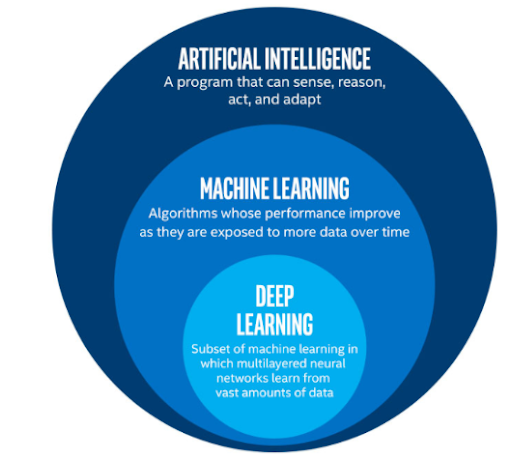
\includegraphics[width=0.47\textwidth]{images/deep_learning/deep_learning_0.png}}

    \caption{Overview of the Artificial Intelligence bubble \cite{Oppermann22}.}
    \label{fig:intro-0}
\end{figure}


More and more companies and organizations are relying on software and automation to become successful. 
Essentially, there is an increasing amount of software that is being pushed to production and this increases 
the number of software vulnerabilities. This gives attackers a bigger playing field for exploiting these 
vulnerabilities which can be catastrophic to many industries so this increases the demand for further improving 
and patching software vulnerabilities. However, with the boom of open-source software community, there an 
abundant amount of code that deep learning (DL) models can learn from in order to detect vulnerable software 
\cite{Lin20}. 

There have been several open-source databases that were created that provides a comprehensive collection of 
software vulnerabilities and defects (Section \ref{sec:data}). This paper is going to cover the different databases that the models 
will use for training and validation. All of the deep learning models in this paper are supervised learning 
models which means they have to learn from some sort of history.

The model that we are going to cover today is the SySeVR framework which is a deep learning model that detects 
software vulnerabilities \cite{Li22}. This will include the datasets it learns from, how its workflow was inspired by 
a computer vision workflow, results, and limitations. Furthermore, this paper is not only going to cover 
SySeVR but it is also going to cover additional frameworks and emphasize the capabilities of deep 
learning for analyzing software. Most importantly, this paper will explain why companies and developers 
should incorporate these existing solutions in the work process so that they push more secure software 
into production and how SySeVR is just one small piece of this puzzle.

% <><><><><><><><><><><><><><><><><><><>
%         DATA - Stefan
% <><><><><><><><><><><><><><><><><><><>
\section{Data}
\label{sec:data}

Databases are extremely important for a wide variety of AI models, especially for deep learning models. 
With the help of the open-source communities organizations were able to create large database for this 
exact purpose.

\subsection{National Vulnerability Database (NVD)}
\label{sub:nvd}

A public repository created by the U.S. government that commonly used for vulnerability management, 
compliance, security measurements, and so on \cite{Nist00}. It has an open-source REST API that can be 
used to provide datasets for deep learning models such as SySeVR to train on (Section \ref{sec:sysevr-framework}).

% <><><><><><><><><><><><><><><><><><><>
%         DEEP LEARNING - Stefan
% <><><><><><><><><><><><><><><><><><><>
\section{Deep Learning (DL)}
\label{sec:deep-learning}

\begin{figure}[t]
    \centering
    \fbox{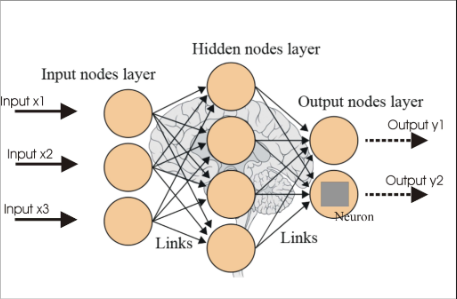
\includegraphics[width=0.47\textwidth]{images/deep_learning/neural_network_0.png}}

    \caption{General architecture of a neural network.}
    \label{fig:dl-0}
\end{figure}

Deep learning (DL) is subset of machine learning that focuses on multi-layered neural networks (NN)
(Figure \ref{fig:intro-0}). Neural networks are inspired by the human brain where the brain learns from 
history or experience and establishes the weights and biases to make decisions. In practice, the neural 
network mimics this exact behavior and is consisted of layers and nodes. NNs can be used for computer vision 
tasks, natural language processing, and pattern recognition.

There are three main layers in an NN: \textbf{input}, \textbf{hidden}, and \textbf{output} layer. 
The input layer of an NN receives the engineered features of a data-point, the outputs of the input layer would
then go through the hidden layer where each node's weight and bias are updated to fit the data-point, and 
then the predictions provided by the output layer (Figure \ref{fig:dl-0}). This is the jist of a 
neural network. However, there are many different types of NNs each of which is tailored for specific 
tasks.

\subsection{Recurrent Neural Network (RNN)}
\label{sub:recurrent-neural-network}

A Recurrent Neural Network (RNN) is a type of NN that contains nodes all of which handles a state from a 
previous timestep, hence, the loops in each node in Figure \ref{fig:dl-1}. This feature allows data to 
persist from one timestep to the next which gives the NN a "Recurrent" nature.

\begin{figure}[h]
    \centering
    \fbox{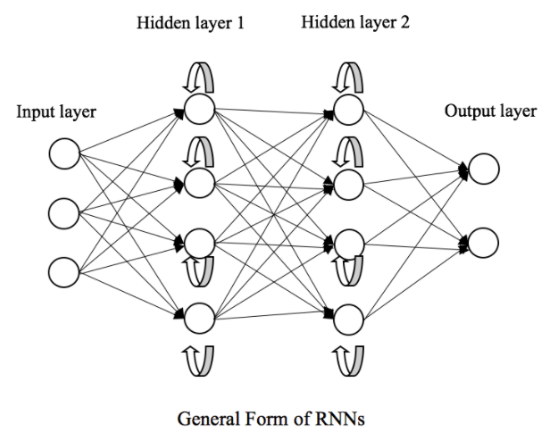
\includegraphics[width=0.47\textwidth]{images/deep_learning/rnn_0.png}}

    \caption{Architecture of a Recurrent Neural Network \cite{Lin20}.}
    \label{fig:dl-1}
\end{figure}

This network is mostly used for natural language processing or data that has a sequential order to it which 
makes an appropriate candidate for learning and detecting software vulnerabilities. 

\subsection{Convolutional Neural Network}
\label{sub:convolutional-neural-network}


\begin{figure}[h]
    \centering
    \fbox{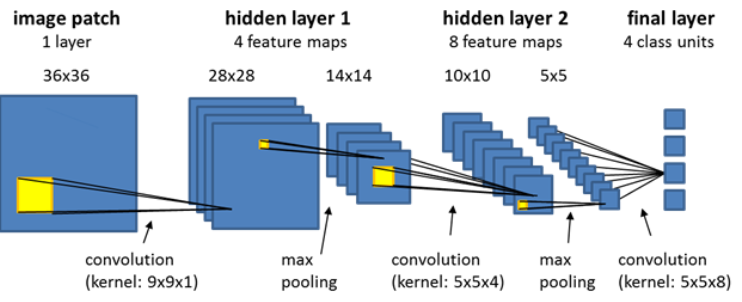
\includegraphics[width=0.47\textwidth]{images/deep_learning/cnn_0.png}}

    \caption{Architecture of a Convolutional Neural Network \cite{Lin20}.}
    \label{fig:dl-2}
\end{figure}


\subsection{Deep Belief Network}
\label{sub:deep-belief-network}

% <><><><><><><><><><><><><><><><><><><>
%          SYSEVR FRAMEWORK - Carter
% <><><><><><><><><><><><><><><><><><><>
\section{SySeVR Framework}
\label{sec:sysevr-framework}

\cite{Li22}

\subsection{Method}
\label{sub:method}

\subsection{Results}
\label{sub:results}

\subsection{Limitations}
\label{sub:limitations}

% <><><><><><><><><><><><><><><><><><><>
%         ADDITIONAL FRAMEWORKS
% <><><><><><><><><><><><><><><><><><><>
\section{Additional Frameworks}
\label{sec:additional-frameworks}

% Carter
\subsection{Automated Vulnerability Detection Machine Using Deep Representation Learning}
\label{sub:automated-vulnerability-detection-machine-using-deep-representation-learning}

\cite{Russell18}

% Carter
\subsection{VulDeBERT: A Vulnerability Detection System Using BERT}
\label{sub:vuldebert}

\cite{Kim22}

% Stefan
\subsection{SAVIOR: Towards Bug-Driven Hybrid Testing}
\label{sub:savior}

\cite{Chen20}

% Stefan
\subsection{VulDeePecker: A Deep Learning-Based System for Multiclass Vulnerability Detection}
\label{sub:vuledeepecker}

\cite{Zou21}

% <><><><><><><><><><><><><><><><><><><>
%         FUTURE WORK - Stefan
% <><><><><><><><><><><><><><><><><><><>
\section{Future Work}
\label{sec:future-work}

\subsection{Working with Version Control}
\label{sub:working-with-version-control}

\subsection{Integrating with CI/CD Pipelines}
\label{sub:integrating-with-cicd-pipelines}

% <><><><><><><><><><><><><><><><><><><>
%          CONCLUSION - Carter
% <><><><><><><><><><><><><><><><><><><>
\section{Conclusion}
\label{sec:conclusion}

% <><><><><><><><><><><><><><><><><><><>
%            REFERENCES
% <><><><><><><><><><><><><><><><><><><>
{\small
\bibliographystyle{ieee_fullname}
\bibliography{egbib}
}

\end{document}
